\section{Historical Evolution}

The journey of special tokens mirrors the evolution of neural sequence modeling itself. From simple boundary markers in early recurrent networks to sophisticated architectural components in modern transformers, special tokens have grown increasingly central to how neural networks process sequential data.

\subsection{Pre-Transformer Era: Simple Markers}

Before transformers revolutionized NLP, special tokens served primarily as boundary markers in recurrent neural networks (RNNs) and their variants. The most common special tokens were:

\begin{itemize}
\item \textbf{Start and End Tokens}: Sequence-to-sequence models used \specialtoken{START} and \specialtoken{END} tokens to delineate generation boundaries
\item \textbf{Unknown Token}: The \specialtoken{UNK} token handled out-of-vocabulary words in fixed vocabulary systems
\item \textbf{Padding Token}: Batch processing required \specialtoken{PAD} tokens to align sequences of different lengths
\end{itemize}

These early special tokens were functional necessities rather than architectural innovations. They solved practical problems but did not fundamentally alter how models processed information.

\subsection{The Transformer Revolution (2017)}

The introduction of the transformer architecture \citep{vaswani2017attention} marked a paradigm shift, though the original transformer used special tokens sparingly. The primary innovation was positional encoding---not technically special tokens but serving a similar purpose of injecting structural information into the model.

\begin{example}[Original Transformer Special Tokens]
The original transformer primarily used:
\begin{itemize}
\item Positional encodings (sinusoidal functions, not learned tokens)
\item \specialtoken{START} token for decoder initialization
\item \specialtoken{END} token for generation termination
\end{itemize}
\end{example}

\subsection{BERT's Innovation: Architectural Special Tokens (2018)}

BERT \citep{devlin2018bert} transformed special tokens from simple markers into architectural components. Three key innovations emerged:

\subsubsection{The [CLS] Token Revolution}
BERT introduced the \cls{} token as a dedicated aggregation point for sentence-level representations. This was revolutionary because:
\begin{itemize}
\item It provided a fixed position for classification tasks
\item It could attend to all positions bidirectionally
\item It eliminated the need for complex pooling strategies
\end{itemize}

\subsubsection{The [SEP] Token for Multi-Segment Processing}
The \sep{} token enabled BERT to process multiple sentences simultaneously, crucial for tasks like:
\begin{itemize}
\item Question answering (question [SEP] context)
\item Natural language inference (premise [SEP] hypothesis)
\item Sentence pair classification
\end{itemize}

\subsubsection{The [MASK] Token and Bidirectional Pre-training}
The \mask{} token enabled masked language modeling (MLM), allowing BERT to learn bidirectional representations. This was impossible with traditional left-to-right language modeling and represented a fundamental shift in pre-training methodology.

\subsection{GPT Series: Minimalist Special Tokens (2018-2023)}

While BERT embraced special tokens, the GPT series \citep{radford2019language} took a minimalist approach:

\begin{itemize}
\item \textbf{GPT-2}: Used only essential tokens like \specialtoken{endoftext}
\item \textbf{GPT-3}: Maintained minimalism but added few-shot prompting patterns
\item \textbf{GPT-4}: Introduced system tokens for instruction following
\end{itemize}

This divergence highlighted a philosophical split: special tokens as architectural components (BERT) versus special tokens as minimal necessities (GPT).

\subsection{Vision Transformers: Cross-Modal Adaptation (2020)}

The Vision Transformer (ViT) \citep{dosovitskiy2020image} demonstrated that special tokens could transcend modalities:

\begin{itemize}
\item Adapted BERT's \cls{} token for image classification
\item Treated image patches as ``tokens'' with positional embeddings
\item Proved that transformer architectures and their special tokens were modality-agnostic
\end{itemize}

\subsection{Multimodal Era: Proliferation and Specialization (2021-Present)}

Recent years have witnessed an explosion in special token diversity:

\subsubsection{CLIP and Alignment Tokens (2021)}
CLIP \citep{radford2021learning} introduced special tokens for aligning visual and textual representations, enabling zero-shot image classification through natural language.

\subsubsection{Perceiver and Latent Tokens (2021)}
The Perceiver architecture introduced learned latent tokens that could process arbitrary modalities, representing a new class of special tokens that are neither input-specific nor task-specific. These innovations built upon efficient transformer research \citep{tay2022efficient}.

\subsubsection{Tool-Use Tokens (2023)}
Models like Toolformer \citep{schick2023toolformer} introduced special tokens for API calls and tool invocation:
\begin{itemize}
\item \specialtoken{Calculator} for mathematical operations
\item \specialtoken{Search} for web queries
\item \specialtoken{Calendar} for date/time operations
\end{itemize}

\subsection{Register Tokens and Memory Mechanisms (2023)}

Recent innovations include register tokens \citep{darcet2023vision} that serve as temporary storage in vision transformers, and memory tokens in models like Memorizing Transformers \citep{wu2022memorizing} that extend context windows through external memory.

\subsection{Timeline of Special Token Innovations}

\begin{figure}[h]
\centering
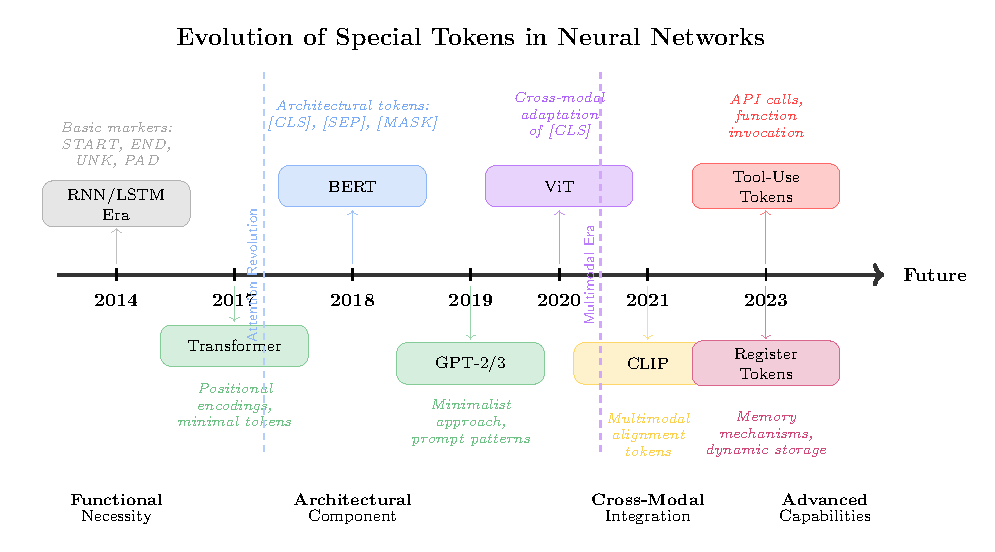
\includegraphics[width=\textwidth]{part1/chapter01/fig_timeline}
\caption{Evolution of special tokens from simple markers to architectural components}
\end{figure}

\subsection{Lessons from History}

The historical evolution of special tokens reveals several important patterns:

\begin{principle}[Evolution Patterns]
\begin{enumerate}
\item \textbf{From Necessity to Architecture}: Special tokens evolved from solving practical problems to enabling new architectures
\item \textbf{Cross-Modal Transfer}: Successful special token designs transfer across modalities (text to vision)
\item \textbf{Task Specialization}: As models tackle more complex tasks, special tokens become more specialized
\item \textbf{Learned vs. Fixed}: The trend moves toward learned special tokens rather than fixed markers
\end{enumerate}
\end{principle}

\subsection{Current Trends and Future Directions}

Today's special token research focuses on:

\begin{itemize}
\item \textbf{Dynamic Tokens}: Tokens that adapt based on input content
\item \textbf{Hierarchical Tokens}: Multi-level special tokens for structured data
\item \textbf{Continuous Tokens}: Soft, continuous representations rather than discrete tokens
\item \textbf{Universal Tokens}: Special tokens that work across different model architectures
\end{itemize}

Understanding this historical context is crucial for appreciating why special tokens are designed the way they are today and for anticipating future developments. As we'll see in subsequent chapters, each major special token innovation has unlocked new capabilities in transformer models, from bidirectional understanding to multimodal reasoning.